\documentclass{article}
\usepackage{amsmath}
\usepackage{amssymb}
\usepackage[table]{xcolor}
\usepackage{tikz}
\usetikzlibrary{positioning}

\begin{document}

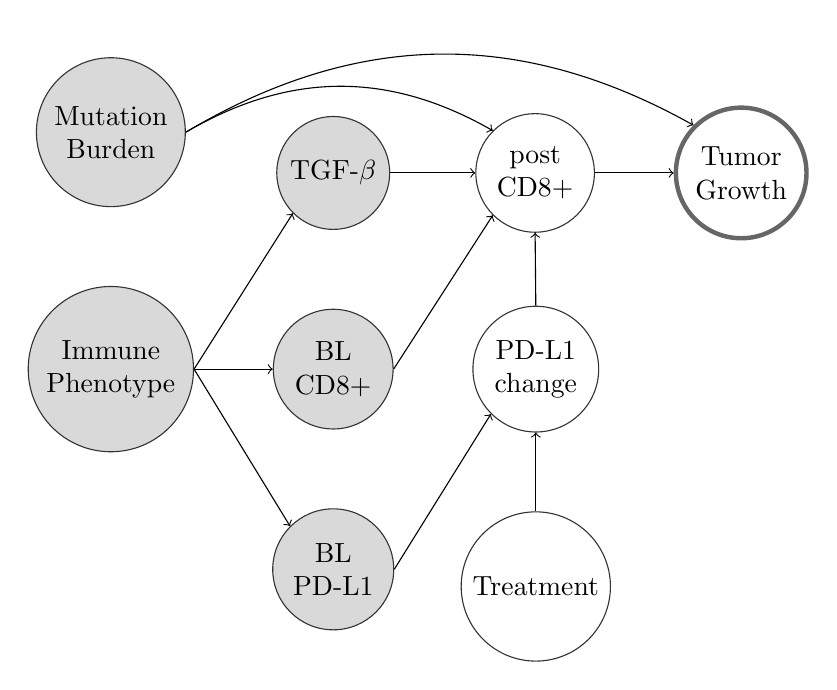
\begin{tikzpicture}[
baseline_node/.style={circle, draw=black!80, fill=gray!30, thin, minimum size=7mm, align=center},
interim_node/.style={circle, draw=black!80, thin, minimum size=7mm, align=center},
target_node/.style={circle, draw=black!60, ultra thick, minimum size=5mm, align=center},
]
%Nodes
\node[baseline_node] (I)                        {Immune\\Phenotype};
\node[baseline_node] (Epre)  [right=of I]       {BL\\CD8+};
\node[baseline_node] (Lpre)  [below=of Epre]    {BL\\PD-L1};
\node[baseline_node] (Bpre)  [above=of Epre]    {TGF-$\beta$};
\node[baseline_node] (M)     [above=of I]       {Mutation\\Burden};
\node[interim_node]  (dL)    [right=of Epre]    {PD-L1\\change};
\node[interim_node]  (Epost) [right=1.08 of Bpre]    {post\\CD8+};
\node[interim_node]  (T)     [below=of dL]      {Treatment};
\node[target_node]   (G)     [right=of Epost]   {Tumor\\Growth};

%Lines
\draw[->] (I.east) -- (Bpre.south west);
\draw[->] (I.east) -- (Lpre.north west);
\draw[->] (I.east) -- (Epre.west);
\draw[->] (Bpre.east) -- (Epost.west);
\draw[->] (Epre.east) -- (Epost.south west);
\draw[->] (Lpre.east) -- (dL.south west);
\draw[->] (T.north) -- (dL.south);
\draw[->] (dL.north) -- (Epost.south);
\draw[->] (M.east) to [bend left] (Epost.north west);
\draw[->] (M.east) to [bend left] (G.north west);
\draw[->] (Epost.east) -- (G.west);

\end{tikzpicture}

\end{document}